\documentclass{article}
\usepackage[utf8]{inputenc}
\usepackage[spanish]{babel}
\usepackage{listings}
\usepackage{graphicx}
\graphicspath{ {images/} }
\usepackage{cite}
\graphicspath{{Images/}}

\begin{document}

\begin{titlepage}
    \begin{center}
        \vspace*{0.2cm}
            
        \Huge
        \textbf{Proyecto de Investigación}
            
        \vspace{0.5cm}
        \LARGE
        Informática II
            
        \vspace{1cm}
            
        \textbf{Daniel Ovany Mesa López}
        
        \vfill
        
        \begin{figure}[htp]
            \centering
            
\includegraphics[width=8cm]{Images/Escudo_UdeA.png}
        \end{figure}
        
            
        \vspace{0.5cm}
            
        \Large
        Despartamento de Ingeniería Electrónica y Telecomunicaciones\\
        Universidad de Antioquia\\
        Medellín\\
        Septiembre de 2020
            
    \end{center}
\end{titlepage}

\tableofcontents

\section{Sección introductoria}
Esta es la primera sección, podemos agregar algunos elementos adicionales y todo será escrito correctamente. Más aún, si una palabra es demasiado larga y tiene que ser truncada, babel tratará de truncarla correctamente dependiendo del idioma.

\section{Sección de contenido} \label{contenido}

Esta sección es para ver qué pasa con los comandos 
que definen texto

El paquete también agrega un comportamiento especial 
a <<estas marcas para hacer citas textuales>> tal como 
lo indican las reglas de la RAE. \cite{dirac}

\begin{lstlisting}
#include <stdio.h>
#define N 10
/* Block
 * comment */

int main()
{
    int i;

    // Line comment.
    puts("Hello world!");
    
    for (i = 0; i < N; i++)
    {
        puts("LaTeX is also great for programmers!");
    }

    return 0;
}
\end{lstlisting}

A continuación se presenta el logo de C++ Figura (\ref{fig:cpplogo})

\begin{figure}[htp]

\includegraphics[width=4cm]{cpplogo.png}
\centering
\caption{Logo de C++}
\label{fig:cpplogo}
\end{figure}

En la sección de teoremas (\ref{contenido})

\section{Conclusión} \label{conclulsion}

\bibliographystyle{IEEEtran}
\bibliography{references}

\vfill

\newpage
\begin{center}
    \title{}
    \textbf{MEMORIA DE UN COMPUTADOR}    
\end{center}
\section*{Introducción:}
\begin{flushleft}
    Un sistema informático es un dispositivo electrónico que consta de dos componentes básicos: hardware y software, puede programarse para realizar diversas operaciones según las necesidades del usuario, necesita de un programa para realizar una operación específica. El sistema operativo asigna los recursos necesarios para ejecutar el programa en términos de espacio de memoria y tiempo de procesamiento de la CPU, esta inicia la ejecución del programa obteniendo la información del sistema de memoria.
    \begin{figure}[htp]
        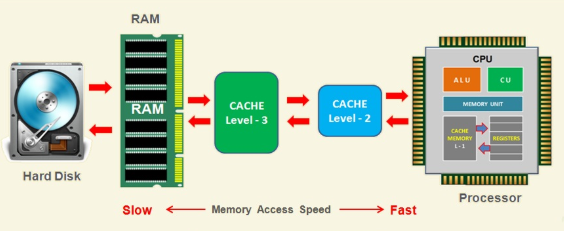
\includegraphics{Images/Sistema de memoria.PNG}
        \caption{Jerarquía de la memoria del sistema de un computador}
        \label{hola:out}
    \end{figure}
    \begin{itemize}
        \item Una memoria es como un cerebro humano, se usa para almacenar información (Datos) o instrucciones (Programas de cómputo), el propósito de almacenamiento es guardar datos que el computador no esté utilizando.
        \item Tipos de memorias:
    \end{itemize}
\end{flushleft}


\end{document}
